\documentclass{article}
\usepackage[utf8]{inputenc}
\usepackage{amsmath}
\usepackage{mathtools}
\usepackage{amsthm}
\usepackage{graphicx}
\usepackage{tabularx}
\usepackage{mathtools}
\usepackage{mathrsfs}
\usepackage{enumerate}
\usepackage{amssymb}
\usepackage{accents}
\usepackage{commath}
\usepackage{yfonts}
\usepackage{float}
\usepackage{array}
\usepackage{tikz-cd}
\usepackage{listings}

\title{Stat3004 Assignment 2}
\author{Dominic Scocchera}
\date{March 2023}

\newtheorem{theorem}{Theorem}
\newtheorem{corollary}{Corollary}
\newtheorem{lemma}[theorem]{Lemma}

\begin{document}
\maketitle
\section*{Q1}
\subsection*{a)}
First we assume that the wallaby is on the integers and starts at 0. Let:
\begin{align*}
P_1&=\mathbb{P}(\text{the wallaby will ever reach x=1})\\
P_u&=\mathbb{P}(\text{the wallaby will ever reach x=u})\\
\end{align*}
By independence we have $(P_1)^u=P_u$. We also have:
\begin{align*}
P_1&=p\cdot1+q\cdot P_2=p+q\cdot(P_1)^2\\
\iff 0&=P_1^2-\frac{1}{q}P_1+\frac{p}{q}\\
\iff P_1&=\frac{1\pm\sqrt{1-4pq}}{2q}\\
&=\frac{1\pm|p-q|}{2q}\\
&=\begin{cases}
1, & \text{if }p\geq q\\
\frac{p}{q}, & \text{if }p<q
\end{cases}
\end{align*}
Hence:
$$P_u=\begin{cases}
1, & \text{if }p\geq q\\
(\frac{p}{q})^u, & \text{if }p<q
\end{cases}$$
\subsection*{b)}
Let $N_{ou}$ denote the time it takes the wallaby to reach $x=u$ for the first time when starting at $x=0$. We now have:
$$\mathbb{E}_u=\mathbb{E}(N_{0u})=u\cdot\mathbb{E}_1$$
Conditioning yields:
$$\mathbb{E}_1=1+p\cdot0+q\cdot\mathbb{E}_2=1+2q\cdot\mathbb{E}_1$$
Now we look at the cases $p<q$, p=q and $p>q$. For $p<q$ we have from a) that $\mathbb{P}(N_{01}=\infty)=1-P_1>0$, implying that $\mathbb{E}_1=\infty$.
\newline\newline
Now for $p=q=\frac{1}{2}$ we get:
$$\mathbb{E}_1=1+\mathbb{E}_1$$
This is a contradiction so $\mathbb{E}_1=\infty$.
\newline\newline
Finally for $p>q$, we get:
$$\mathbb{E}_1=\frac{1}{1-2q}=\frac{1}{p-q}$$
Hence:
$$\mathbb{E}_u=\begin{cases}
\infty & \text{if } p\leq q\\
\frac{u}{p-q} & \text{if } p>q
\end{cases}$$
And so the expected moves when $p=q=\frac{1}{2}$ is $\infty$.
\subsection*{e)}
With almost identical working out to a) we can get:
$$P_d=\begin{cases}
1, & \text{if }p\leq q\\
(\frac{q}{p})^d, & \text{if }p>q
\end{cases}$$
So the probability of ever reaching the seeds ($P_s$) is:
$$P_s=P_u \text{ or } P_d=\begin{cases}
P_d=P_u=1, & \text{if }p= q\\
P_u=(\frac{p}{q})^u,\;\;P_d=1, & \text{if }p<q\\
P_u=1,\;\;P_d=(\frac{q}{p})^d, & \text{if }p>q
\end{cases}$$
So no matter what p and q are the wallaby is guaranteed to reach some seeds.
\subsection*{f)}
With almost the exact same working out as in b) we can get:
$$\mathbb{E}_d=\begin{cases}
\infty & \text{if } p\geq q\\
\frac{|d|}{q-p} & \text{if } p<q
\end{cases}$$
Now we get:
\begin{align*}
\mathbb{E}_s&=\begin{cases}
\mathbb{E}_u=\mathbb{E}_d=\infty & \text{if } p=q\\
\mathbb{E}_u=\frac{u}{p-q},\;\;\mathbb{E}_d=\infty & \text{if } p>q\\
\mathbb{E}_u=\infty,\;\;\mathbb{E}_d=\frac{|d|}{q-p} & \text{if } p<q
\end{cases}\\
&=\begin{cases}
\infty & \text{if } p=q\\
\frac{u}{p-q} & \text{if } p>q\\
\frac{|d|}{q-p} & \text{if } p<q
\end{cases}\\
\end{align*}
\section*{Q2}
\subsection*{a)}
\begin{center}
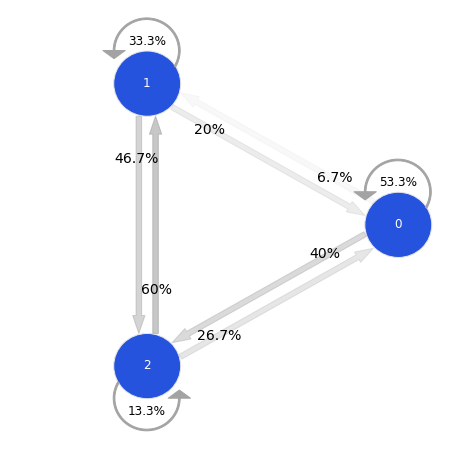
\includegraphics[scale=0.5]{markov.png}
\end{center}
\subsection*{b)}
\begin{align*}
\mathbb{P}(X_3=1|X_0=1)&=\mathbb{P}(X_3=1|X_0=1,X_1=0,X_2=0)+\mathbb{P}(X_3=1|X_0=1,X_1=0,X_2=1)\\
&+\mathbb{P}(X_3=1|X_0=1,X_1=0,X_2=2)+\mathbb{P}(X_3=1|X_0=1,X_1=1,X_2=0)\\
&+\mathbb{P}(X_3=1|X_0=1,X_1=1,X_2=1)+\mathbb{P}(X_3=1|X_0=1,X_1=1,X_2=2)\\
&+\mathbb{P}(X_3=1|X_0=1,X_1=2,X_2=0)+\mathbb{P}(X_3=1|X_0=1,X_1=2,X_2=1)\\
&+\mathbb{P}(X_3=1|X_0=1,X_1=2,X_2=2)\\
&=\frac{3}{15}\frac{8}{15}\frac{1}{15}+\frac{3}{15}\frac{1}{15}\frac{5}{15}+\frac{3}{15}\frac{6}{15}\frac{9}{15}+\frac{5}{15}\frac{3}{15}\frac{1}{15}+\frac{5}{15}\frac{5}{15}\frac{5}{15}+\frac{5}{15}\frac{7}{15}\frac{9}{15}\\
&+\frac{7}{15}\frac{4}{15}\frac{1}{15}+\frac{7}{15}\frac{9}{15}\frac{5}{15}+\frac{7}{15}\frac{2}{15}\frac{9}{15}\\
&=\frac{1}{3}\\
\end{align*}
\subsection*{c)}
To find the limiting distribution we solve $\pi(P-I)=\bold{0}$.
\begin{lstlisting}
import numpy as np
from scipy . linalg import null_space

P = (1/15)*np.array([[8, 1, 6], [3, 5, 7], [4, 9, 2]])
v = null_space(P - np.eye(3))
v = v/sum(v)
\end{lstlisting}
From this we find that $\pi=\left(\frac{1}{3},\frac{1}{3},\frac{1}{3}\right)^T$.
\section*{Q3}
\subsection*{a)}
We want to show that for $x,y\in E$, if $x\rightarrow y$ but $r_{yx}=\mathbb{P}_y(\tau_y<\infty)<1$ (i.e. $y\nrightarrow x$) then x is transient.
\begin{proof}
First consider the probability that we return to y after time n conditioned on whether or not $X_n=y$.
\begin{align*}
\mathbb{P}(\text{return to x after time n}|X_0=x)&=r_{xy}\mathbb{P}(\text{return to x after time n}|X_n=y,X_0=x)\\
&+(1-r_{xy})\mathbb{P}(\text{return to x after time n}|X_n\neq y,X_0=x)\\
&\leq 0+(1-r_{xy})\\
&<1\\
\end{align*}
As $\mathbb{P}(\text{return to x after time n}|X_0=x)<1$ then x must be transient (if it were recurrent it would equal 1 as we would be able to return infinitely often). We also note here that $\mathbb{P}(\text{return to x after time n}|X_n=y,X_0=x)=0$ as we can't return to x from y and $\mathbb{P}(\text{return to x after time n}|X_n\neq y,X_0=x)\leq 1$ as there exists at least one state namely y that makes it impossible to return to x.
\end{proof}
\section*{Q4}
\subsection*{a)}
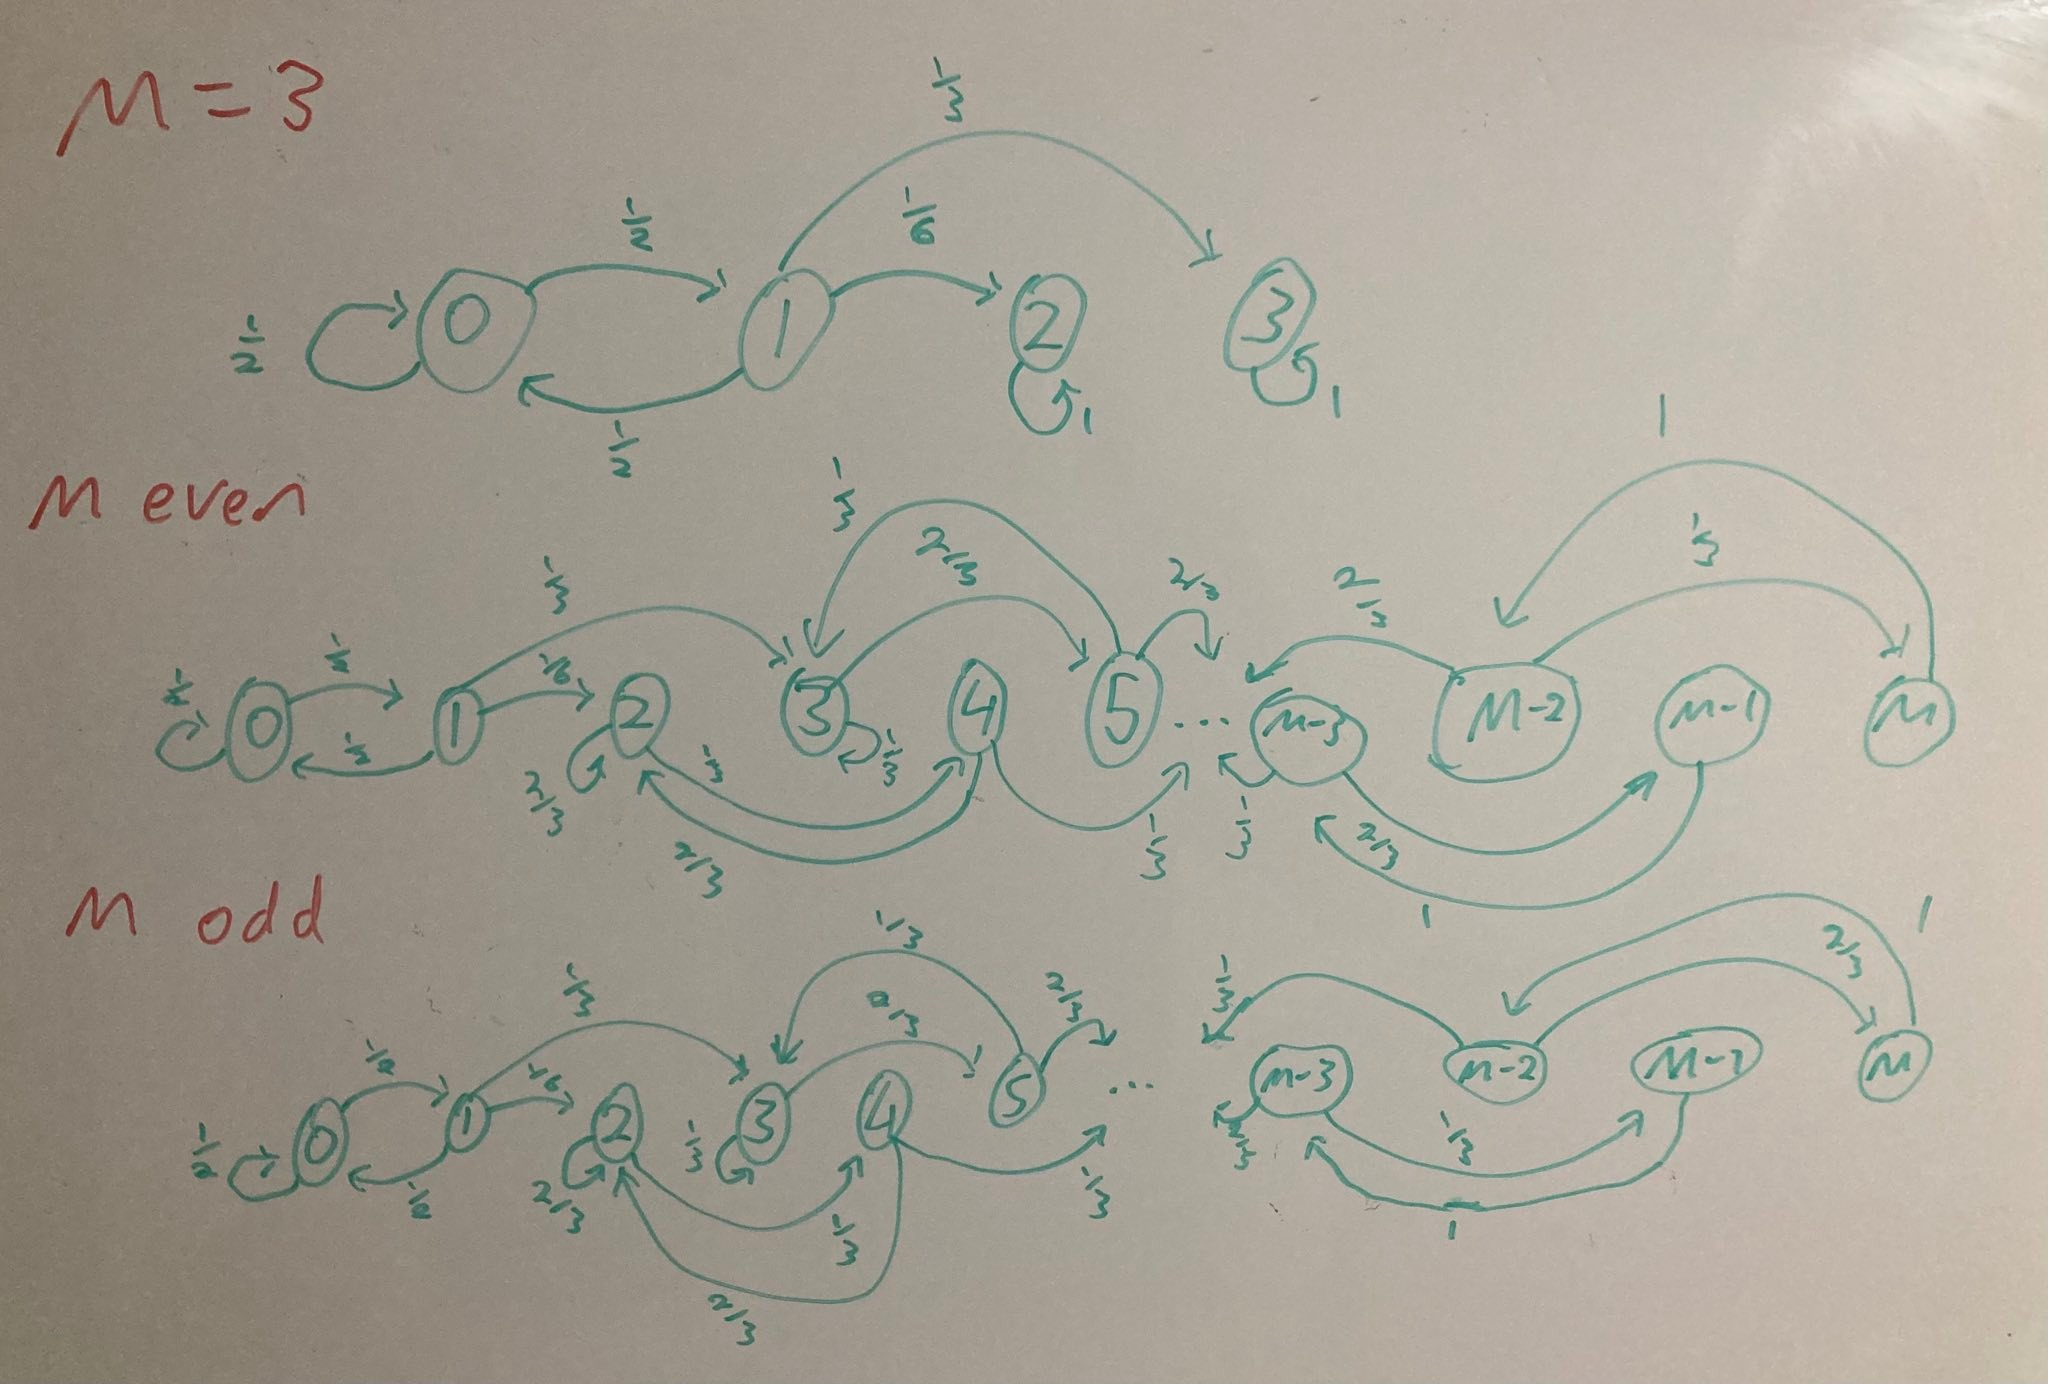
\includegraphics[scale=0.2]{a2q4.jpeg}
\subsection*{b)}
There are three communicating classes, $A=\{0,1\}$, $B=\{2i\;\;|\;\;2\leq 2i\leq M\}$ (even integers greater or equal to 2) and $C=\{2i+1\;\;|\;\;3\leq2i+1\leq M\}$ (odd integers greater or equal to 3).
\subsection*{c)}
We have three cases:
\newline
M=3:
\newline
A is transient. B is closed, recurrent and absorbing. C is closed, recurrent and absorbing.
\newline
M=4:
\newline
A is transient. B is closed and recurrent. C is closed, recurrent and absorbing.
\newline
$M>4$:
\newline
A is transient. B is closed and recurrent. C is closed and recurrent.
\subsection*{d)}
First we note that as A is transient, so it is always aperiodic.
\newline\newline
We have four cases:
\newline
M=3:
\newline
2 is absorbing so the period is 1 which makes it aperiodic by definition. Same for 3.
\newline
M=4:
\newline
3 is absorbing so the period is 1 which makes it aperiodic by definition. Starting at 2 we return to 2 after either 1 or 2 transitions, $\delta_x=\text{gcd}(1,2)=1$, so 2 is aperiodic. $2\leftrightarrow4$ so 4 is also aperiodic.
\newline
$M=5$:
\newline
Starting at 2 we return to 2 after either 1 or 2 transitions, $\delta_x=\text{gcd}(1,2)=1$, so 2 is aperiodic. $2\leftrightarrow4$ so 4 is also aperiodic. Starting at 3 we return to 3 after either 1 or 2 transitions, $\delta_x=\text{gcd}(1,2)=1$, so 3 is aperiodic. $3\leftrightarrow5$ so 5 is also aperiodic.
\newline
$M>5$:
\newline
We note that $p_{22}=\frac{2}{3}>0$ and $p_{33}=\frac{1}{3}>0$. From lectures we know that this means 2 and 3 must be aperiodic. We also know that if $x\leftrightarrow y$ then x and y have the same period. So all states in B and C must be aperiodic.
\end{document}